%\documentclass[pldi]{sigplanconf-pldi16}
\documentclass[sigconf, anonymous]{acmart}


%\documentclass[letterpaper,twocolumn,10pt]{article}
%\usepackage{usenix2019_v3_hotos}
% standard LaTeX packages
%\usepackage{changebar}

\usepackage{balance}
\usepackage{alltt}
\usepackage{amsmath}
\usepackage{balance}
\usepackage{booktabs}
\usepackage{fixltx2e}
\usepackage{graphicx}
\usepackage{boxedminipage}
\usepackage{hyperref}
\usepackage{nicefrac}
\usepackage{subfigure}
%\usepackage{xcolor}
\usepackage{setspace}
\usepackage{xspace}
\usepackage{multirow}
\usepackage{colortbl}
\usepackage{amsfonts} 
\usepackage{blindtext}
\usepackage{chngpage}
\usepackage{listings}
\usepackage{color}
%\usepackage[dvipsnames]{xcolor}
\usepackage{mathtools}
\usepackage{amssymb}
\usepackage{pifont}
%\usepackage[numbers,sort&compress,square]{natbib}

\usepackage{array}
\newcolumntype{x}[1]{>{\centering\arraybackslash\hspace{0pt}}p{#1}}


\settopmatter{printacmref=false}

\captionsetup{format=default, font=bf}





%% taken from unknown.sty
%\DeclareCaptionType{copyrightbox}

\sloppy

\input macros.tex

\begin{document}

%\newcommand{\vt}{VirusTotal}
\title{Understanding Real-World Malwares and Anti-Virus Engines}


\maketitle


%\theoremstyle{definition}
%\newtheorem{definition}{Definition}[section]

\begin{abstract}
ToDO
\end{abstract}

\section{Introduction}

\textcolor{gray}{Combating malware is important.} 

Malwares threaten information facilities and cause a large amount of loss each year. Anti-malware tools improve rapidly to detect malwares. 
Nowadays, there are also online malware analysis services for malware detection, such as VirusTotal \cite{VirusTot68:online}. 
VirusTotal allows users to submit suspicious samples, and offers detection results for tens of anti-virus vendors.
VirusTotal has become an important platform for both anti-malware industry and academia.

Combating malware needs efforts from the whole community. VirusTotal is a website, combining vendors? new detection techniques. VirusTotal is widely used in industry.

Beyond industry, academia also widely uses VirusTotal for different purposes. 

Our measurement shows that research community is using VirusTotal in a wrong way. 

VirusTotal is used in a wrong way. 

The question we want to ask is whether academia uses VirusTotal in a correct way. If not, how should we use VirusTotal. 

Contribution:

a. We survey more than 100 academic paper and summarize how researchers use VirusTotal. We find two usage patterns.

b. We collect big data from VirusTotal and use these data to show that the current usage of VirusTotal is wrong. 

c. We build a prediction model to help better use VirusTotal


\section{\vt\ Usage Study}

In this section, we present the empirical study on how 
academic people use \vt. 
We will first discuss how we collect academic papers to conduct the study, 
and then we will present our findings and implications. 

\subsection{Methodology}

We leverage published academic papers to understand 
how academic people use \vt,
since published papers usually contain detailed descriptions 
about how the authors use \vt\ in their projects, if \vt\ is involved. 

To collect academic papers, we search for keyword ``\vt'' in Google Scholar. 
In total, we find 101 conference papers published in the last ten years.
We then manually inspect descriptions related to \vt\ in these papers. 
In 87 papers, the authors either use \vt\ 
to build a data set for their evaluation~\cite{ford2009analyzing,android-1,email-vt-1,kharraz2016unveil} 
or leverage querying \vt\ as one building block of their
techniques~\cite{vt-component-1,vt-component-2,vt-component-3}. 
These 87 papers are targets of our \vt{} usage study. 
For the left 14 papers, their authors just discuss \vt\ as a part 
of technical background~\cite{not-use-1,bayer2009scalable,jiang2012dissecting}, and 
they do not use \vt\ in building their techniques or evaluation. 
Therefore, we ignore these papers in our study. 


\begin{figure}%
\centering
\subfigure[Conference]{%
\label{fig:conference}%
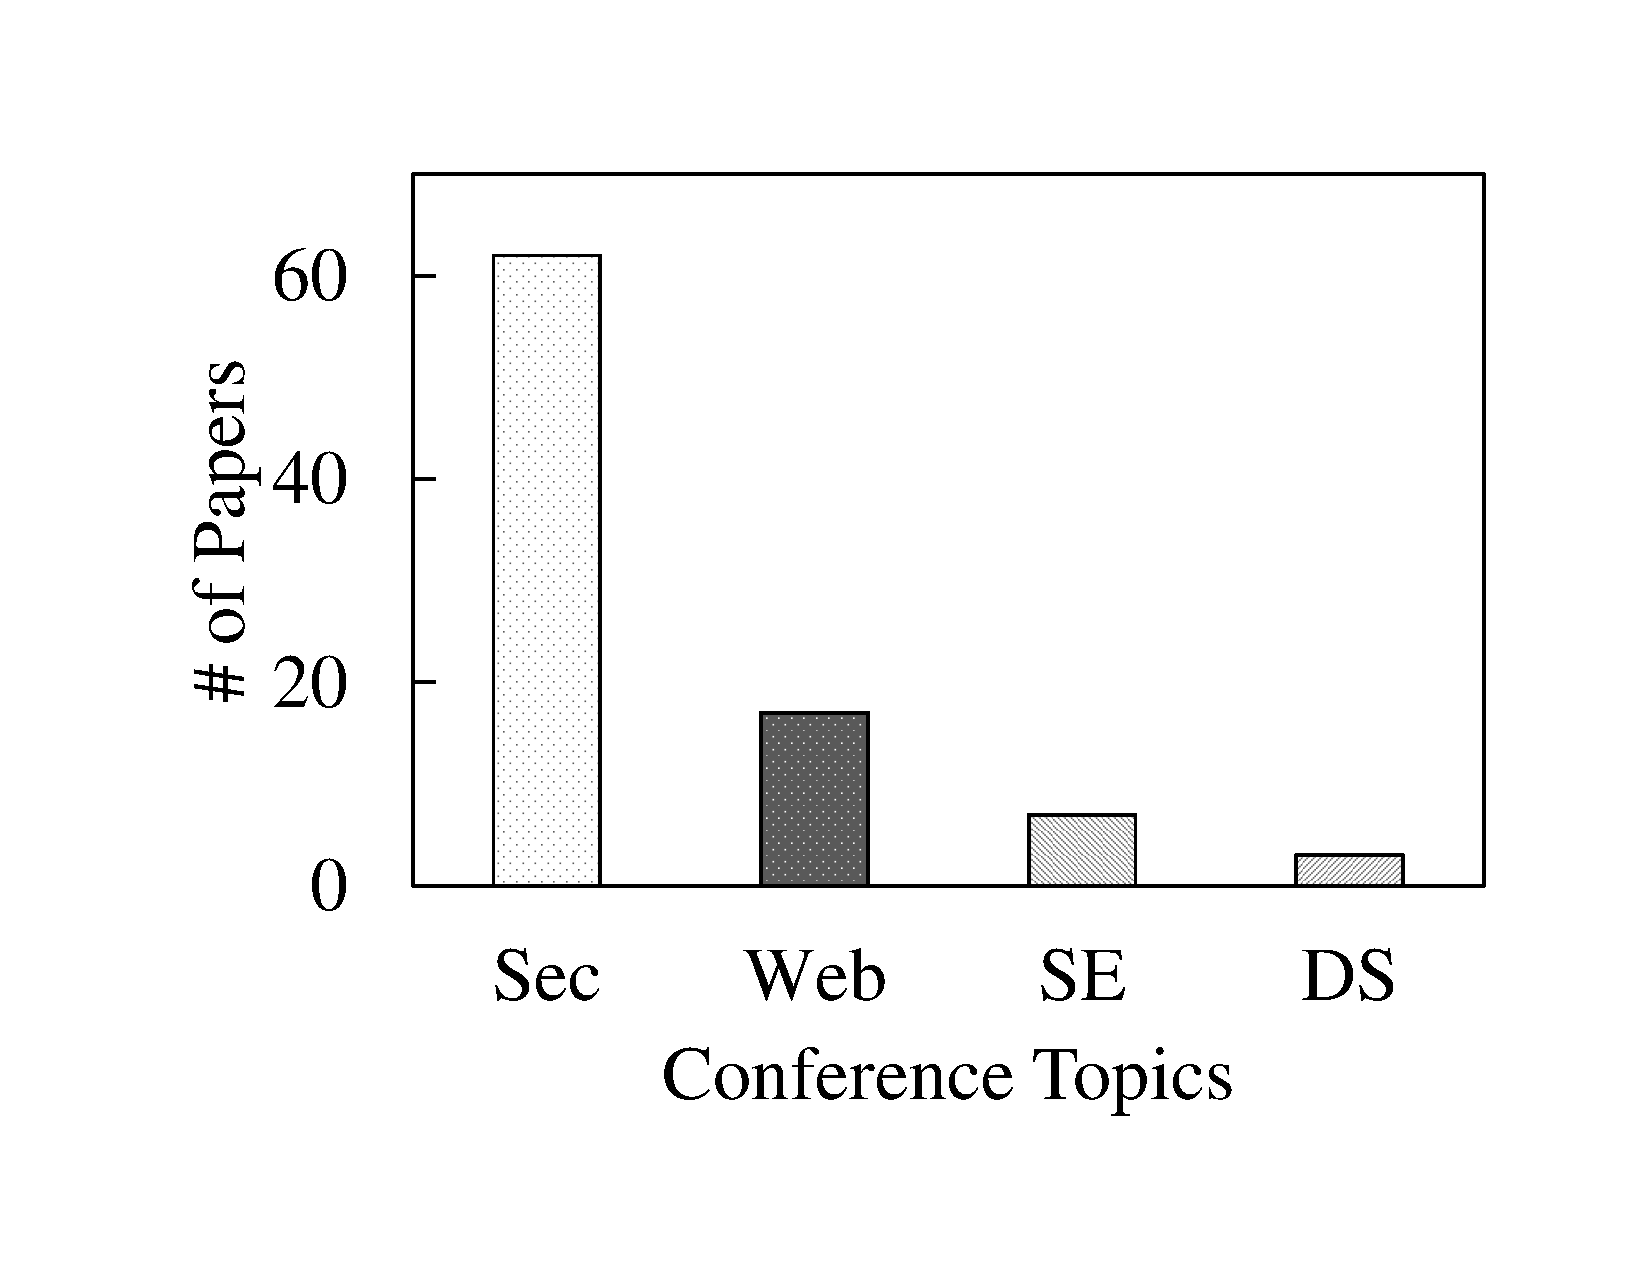
\includegraphics[width=1.45in]{figure/literature-confs}}%
\qquad
\subfigure[Publication Year]{%
\label{fig:year}%
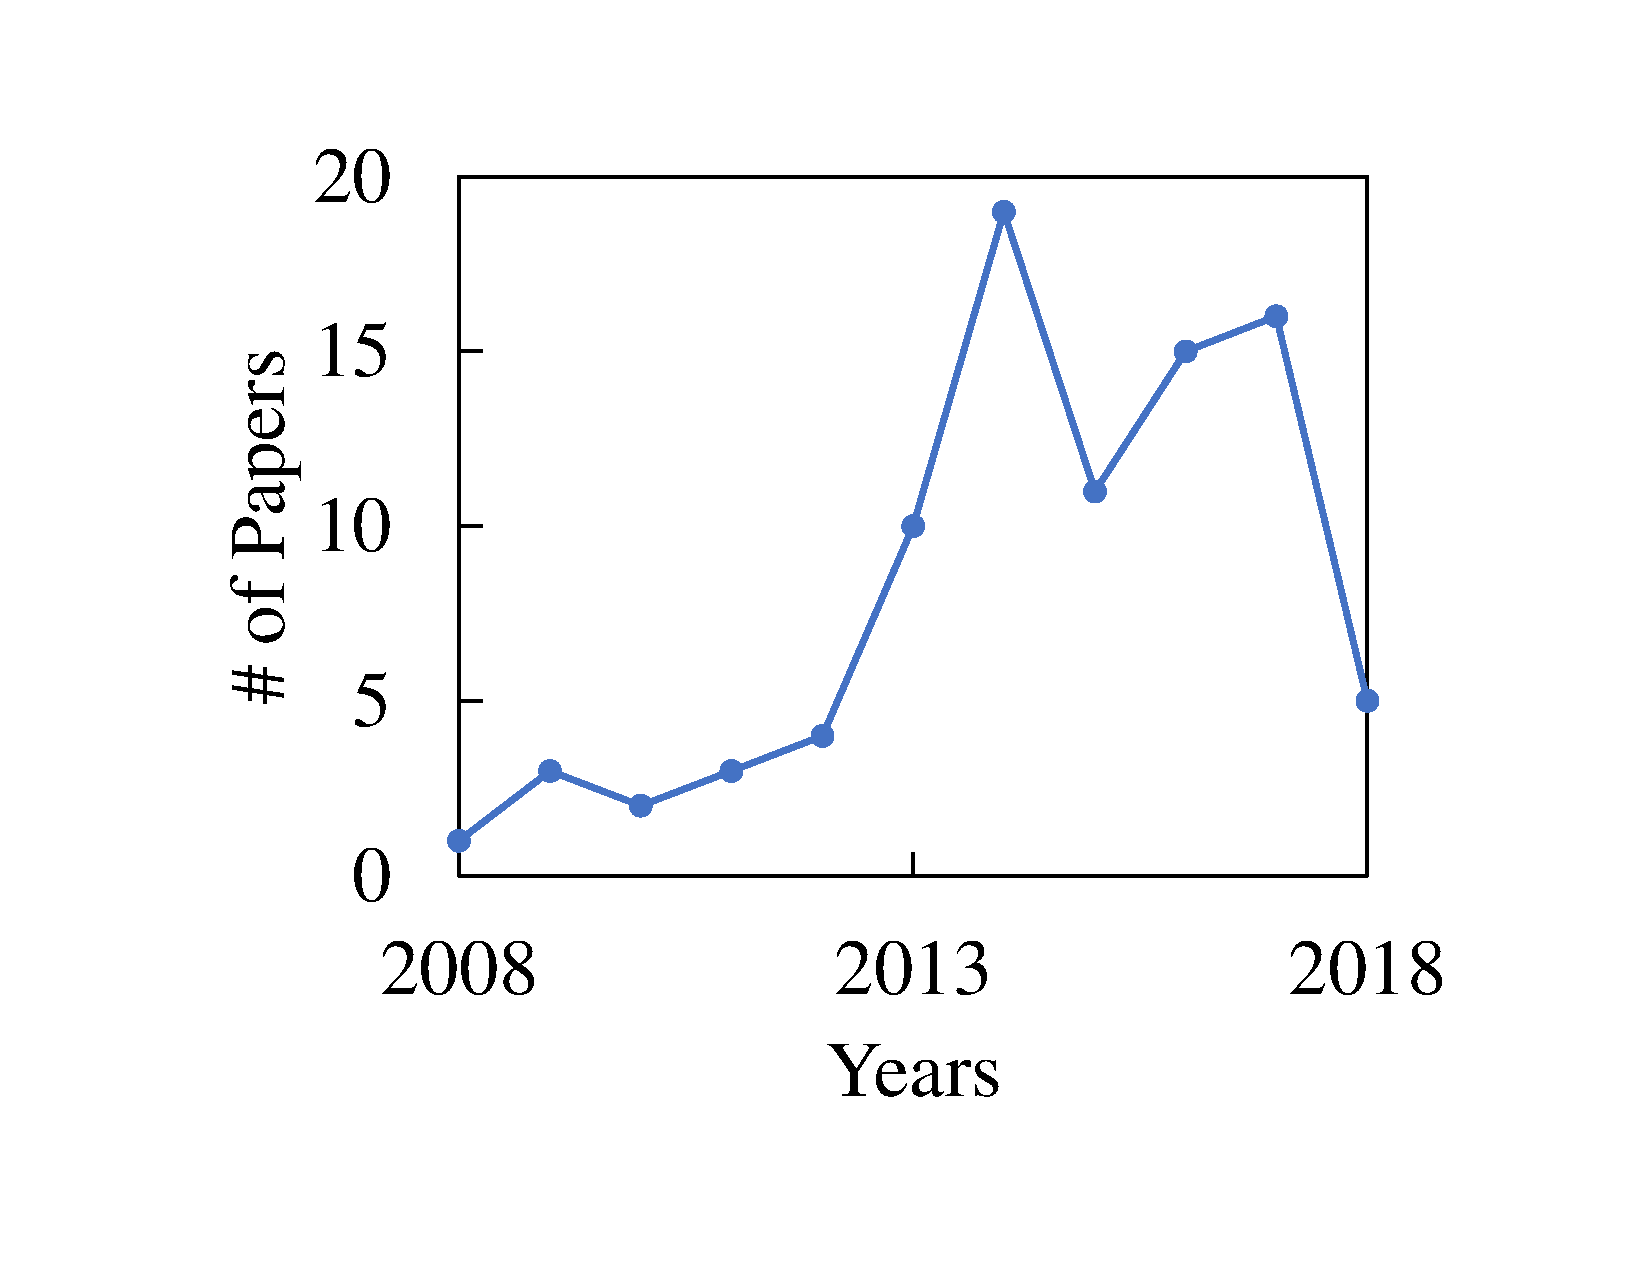
\includegraphics[width=1.45in]{figure/literature-years}}%
\mycaption{fig:char}
{Characteristics of our studied papers.}
{Sec: Security, DS: Data Science and SE: Software Engineering.}
\end{figure}




As shown in Figure~\ref{fig:conference}, 
our collected papers mainly come from famous academic conferences 
in four research areas, security, software engineering, data science, and web. 
For example, in total, we study 62 papers published in security conferences,
and 28 of them come from the top four security conferences, 
IEEE S\&P, CCS, Usenix Security, and NDSS.
As shown in Figure~\ref{fig:year}, 
we have at least one studied papers 
published in each year from 2008 to 2018. 
19 studied papers are published in 2014, 
and it is the year with largest number. 
Our studied papers cover different types of malware, 
such as Android APK~\cite{android-1,arp2014drebin,huangvt2016bigdata}, 
Portable Executable (PE) files~\cite{bayer2009scalable,pe-vt-1,pe-vt-2}, 
Flash~\cite{ford2009analyzing,wressnegger2017looking}, 
PDF~\cite{pdf-vt-1,carmony2016extract}, and so on. 
To sum up, we believe our studied paper is a representative data set 
to understand how academic people use \vt{}. 

\subsection{Findings and Implications}
We mainly want to answer two questions through our study.
First, \vt{} applies multiple antivirus engines to scan every submitted file, 
and returns all detection results to user.
Different engines may disagree with each other.
We want to understand how academic users aggregate results from different vendors,
and make the decision about whether a submitted file is benign for malicious. 
Second, \vt{} keeps updating antivirus engines. 
Intuitively, detection results could change when the same file is submitted twice.
We want to know whether or not academic users consider 
possible result changes on \vt{} over time.   
 

\noindent{\underline{How detection results are merged?}}
For 72 out of 89 (80.89\%) studied papers, 
their authors leverage a threshold to decide whether a submitted file is 
malicious or not. 
The threshold can either be a absolute number, 
or a ratio of the number of engines with malicious labels over all engines.
There are 26 studied papers, 
whose authors consider a submission is malicious, 
if any vendor label it as malware. 
For another {\color{red} XXX} papers, their authors 
use a absolute threshold number that is larger than one. 
Authors of {\color{red} XXX} papers use a ratio as their threshold. 
For the left 17 papers, their descriptions about how to merge results 
is not clear enough for us to study. 


\noindent{\underline{Whether possible changes are considered?}}





There several issues that researchers need to consider in using the results. 
First, researchers could collect detection results from multiple vendors. 
It is necessary to aggregate the results into one as the label of malware or benign for some works. 
We would like to know how researchers aggregate them. 
Second, the detection results could change over time and it is more reliable to collect the results from \vt\ during a period of time. 
We would also like to know the practice on collecting results from \vt\ over time. 
Thrid, vendors could have different impacts. 
It is also interesting to know whether and how researchers considered the different impacts of vendors.

%Last but not least, it is worth considering how we merge results from different vendors. 
First, we look at how researchers merge detection results. 
In most cases, researchers get results from more than 40 or 50 vendors and merge the results as one for their dataset. 
There are mainly two ways of merging: 1) considering a submission as malicious if any vendor can detect; 2) considering a ratio or a threshold for the number of vendors. 
For instance, Ford et al. \cite{ford2009analyzing} report it as malicious as long as there is a vendor reporting malicious
towards a file, while Carmony et al. use a threshold of 15 files. 
Among the 89 papers, 26 papers (29.2\%) use the first way and 46 papers  (51.7\%) use the second way. 
The rest 17 papers (19.1\%) do not mention how they merge results from different vendors.

Second, there are only 4 papers (4.5\%) consider that the detection results could change over time, and collect the results from \vt\ during a period of time. 
The length of time could vary from several days \cite{kharraz2016unveil, rajab2013camp} to months \cite{neeles, wressnegger2017looking}. 

Third, among the 89 papers, only 8 papers (9.0\%) consider that different vendors shall have different impact. 
Most of them pick out three to more than ten vendors to discuss their impact, because of their influence in industry or good performance on detection rate. 
For instance, Arp et al. \cite{arp2014drebin} inspected the output of ten vendors and list their detection rate anonymously. 
In addition, all of the papers treat the vendors equally. %Thomas et al. \cite{thomas2015ad} listed detection rate of 3 vendors. 
\subsection{Findings}
a. Do not wait until results become stable

b. Treat vendors equally

\subsection{Discussion}
What if the current usage is not correct? 

\section{Data Collection and Basic Analysis}
\label{sec:data}

This section introduces \vt{} and how we collect data from \vt{}. 
We also conduct simple analysis to understand 
the basic properties of our collected data. 

\subsection{\vt{}}
\vt{} is a free online malware scan service. 
It was founded in 2004 and was acquired by google in 2012. 
\vt{} is widely used anti-virus vendors to identify false positives and false negatives 
in their products~\cite{huangvt2016bigdata, neeles}, 
and individual users, including many academic people 
as we discussed in Section~\ref{sec:label}.

For each submitted sample, \vt applies a set of anti-virus engines to analyze it. 
\vt{} keeps information about whether the submission is labeled as malware by each engine, 
and detailed tags for identified malware from each engine. 

For each submitted sample, \vt applies a set of anti-virus engines to analyze it. 
\vt{} keeps information about whether the submission is labeled as malware by each engine, 
and detailed tags for identified malware from each engine. 
\vt{} provides open APIs for users to interact with \vt{} 
and access the metadata of all submissions and latest detection results.
For example, \texttt{rescan} api asks \vt{} to analyze a previously submitted file again. 
\texttt{report} api returns detailed metadata and latest detection results for a file as shown in Table~\ref{xxx}. 
\texttt{distribution} api works like a pipe and keeps 
downloading information for latest submitted data from \vt{}. 



\subsection{Data Collection}

First, we introduce our data source, VirusTotal, and how we make use of their APIs. VirusTotal offers a lot of APIs for researchers. Their private APIs could return the detailed detection results of vendors. We applied for a private API key for our data collection. We mainly use two APIs for collecting data: \texttt{report} and \texttt{rescan}. \texttt{report} takes a hash value of a sample as input, and returns a detailed report of the sample if the sample exists in the library of VirusTotal. The report contains the detection results of the sample from all the vendors that VirusTotal could provide. \texttt{rescan} also takes a hash value as input. This API sets VirusTotal to rescan the specified sample. This could make VirusTotal to update the detection results of samples.

Then we introduce how to collect the data set. 
First, at day 0, we obtained about 14,423 new Portable Executable (PE, the executable file format on Windows) files from an anti-virus vendor. 
We then submitted the 14423 files to VirusTotal at the same day, and got the detection results from VirusTotal. 
None of these files were submitted to VirusTotal prior to day 0.
For each day later on, we first call \texttt{rescan} on the 14423 files respectively. Then, we wait 2 hours for VirusTotal updating the detection results. 
After 2 hours, we call \texttt{report} on each files to get the updated detection results. 
We keep collecting data for 75 days. 


\begin{table}[h!]
\centering
\footnotesize
{
\begin{tabular}{l|l}
\hline
Metadata Field & Explanation \\
\hline                            
%\cline{1-1}
{\bf name}      & submitted file name \\
{\bf link}      & where to download the file \\
{\bf timestamp} & timestamp when the submission was made \\
{\bf source\_country} & the country where the submission was made \\
{\bf source\_id} & user ID who made the submission\\
{\bf size} & file size \\
{\bf type} & file type \\
{\bf tags} & labels with more specific information for each {\bf type}\\
{\bf first\_seen} & when the same file was first submitted \\
{\bf last\_seen} & when the same file was last submitted \\
{\bf hashes} & sha1, sha256, md5, and vhash\\
{\bf ssdeep} & ssdeep digest string \\
{\bf total} & number of engines analyzing the file \\
{\bf positives} & number of engines that flagged the file as malicious \\
{\bf positives\_delta} & changes in {\bf positives} across different submissions\\
{\bf report} & detailed detection report from each AV engine \\
\hline
\end{tabular}
}
\caption{VirusTotal Metadata. 
%\footnotesize{
(Fields for each submission retrieved from VirusTotal through distribution API and their related explanation.
One file could be submitted multiple times by different users.)
%}
}
\label{tab:fields}
\end{table}


\subsection{What information can we get from VirusTotal?}% I mean the data format. 

The API \texttt{report} returns a lot of information of the sample, including but not limited to hashcodes (MD5, SHA1, etc.) of the sample, scan date, and detailed scan results of many vendors. For each vendor in the detailed scan results, there are 4 fields: \texttt{detected}, \texttt{version}, \texttt{result}, and \texttt{update}. \vt\ does not provide detailed documentation of the fields, but it is easy to infer from the results and other documents (such as https://www.virustotal.com/en/faq/). \texttt{detected} tells if the sample is detected as malicious by this vendor. \texttt{version} tells the version used in the scan. \texttt{result} is how the vendor classifies the sample. \texttt{update} is the date of the vendor providing the anti-virus tool.

\subsection{Basic properties of the data set}

Now we take a look at the data set. First, there are 7197 malicious files and 7226 benign files according to the results from first scan. We say ``malicious'' as long as there is one vendor reporting malicious. This indicates that our dataset is balanced.

Then we check the completeness of the dataset by observing two distributions. 
Our dataset could be regarded as a set of tuples $(f, v, t)$ that sample $f$ is scanned at time $t$ by vendor $v$. Ideally, there should be one tuple for all $f, v, $ and $t$ in all 14423 files, more than 70 vendors and 75 days. 
However, not all valid tuples exist in the downloaded information. Some tuples may miss because of VirusTotal or our crawling configuration. So we calculated two distributions of the data set to check the completeness.
First, Figure~\ref{fig:dataset_submission_vendor_distri} shows the distribution of how many vendors have scanned a sample in a detection result. A point $(x, y)$ on the curve represents that there are $y$ detection results with $x$ vendors scanned. From the chart, we can know that most of the detection results are detected by more than 65 vendors. 
In addition, Figure~\ref{fig:dataset_no_vendors_scanned_moste_files_in_x_days} shows  how many vendors scan most of the files in how many days. More specifically, $(x, y)$ in the chart represents there are $y$ vendors that scans more than 90\% of the total files in $x$ days. The figure indicates that most of the vendors 
From the two figures, we could conclude that the dataset is mostly complete.

\begin{figure}
\centering
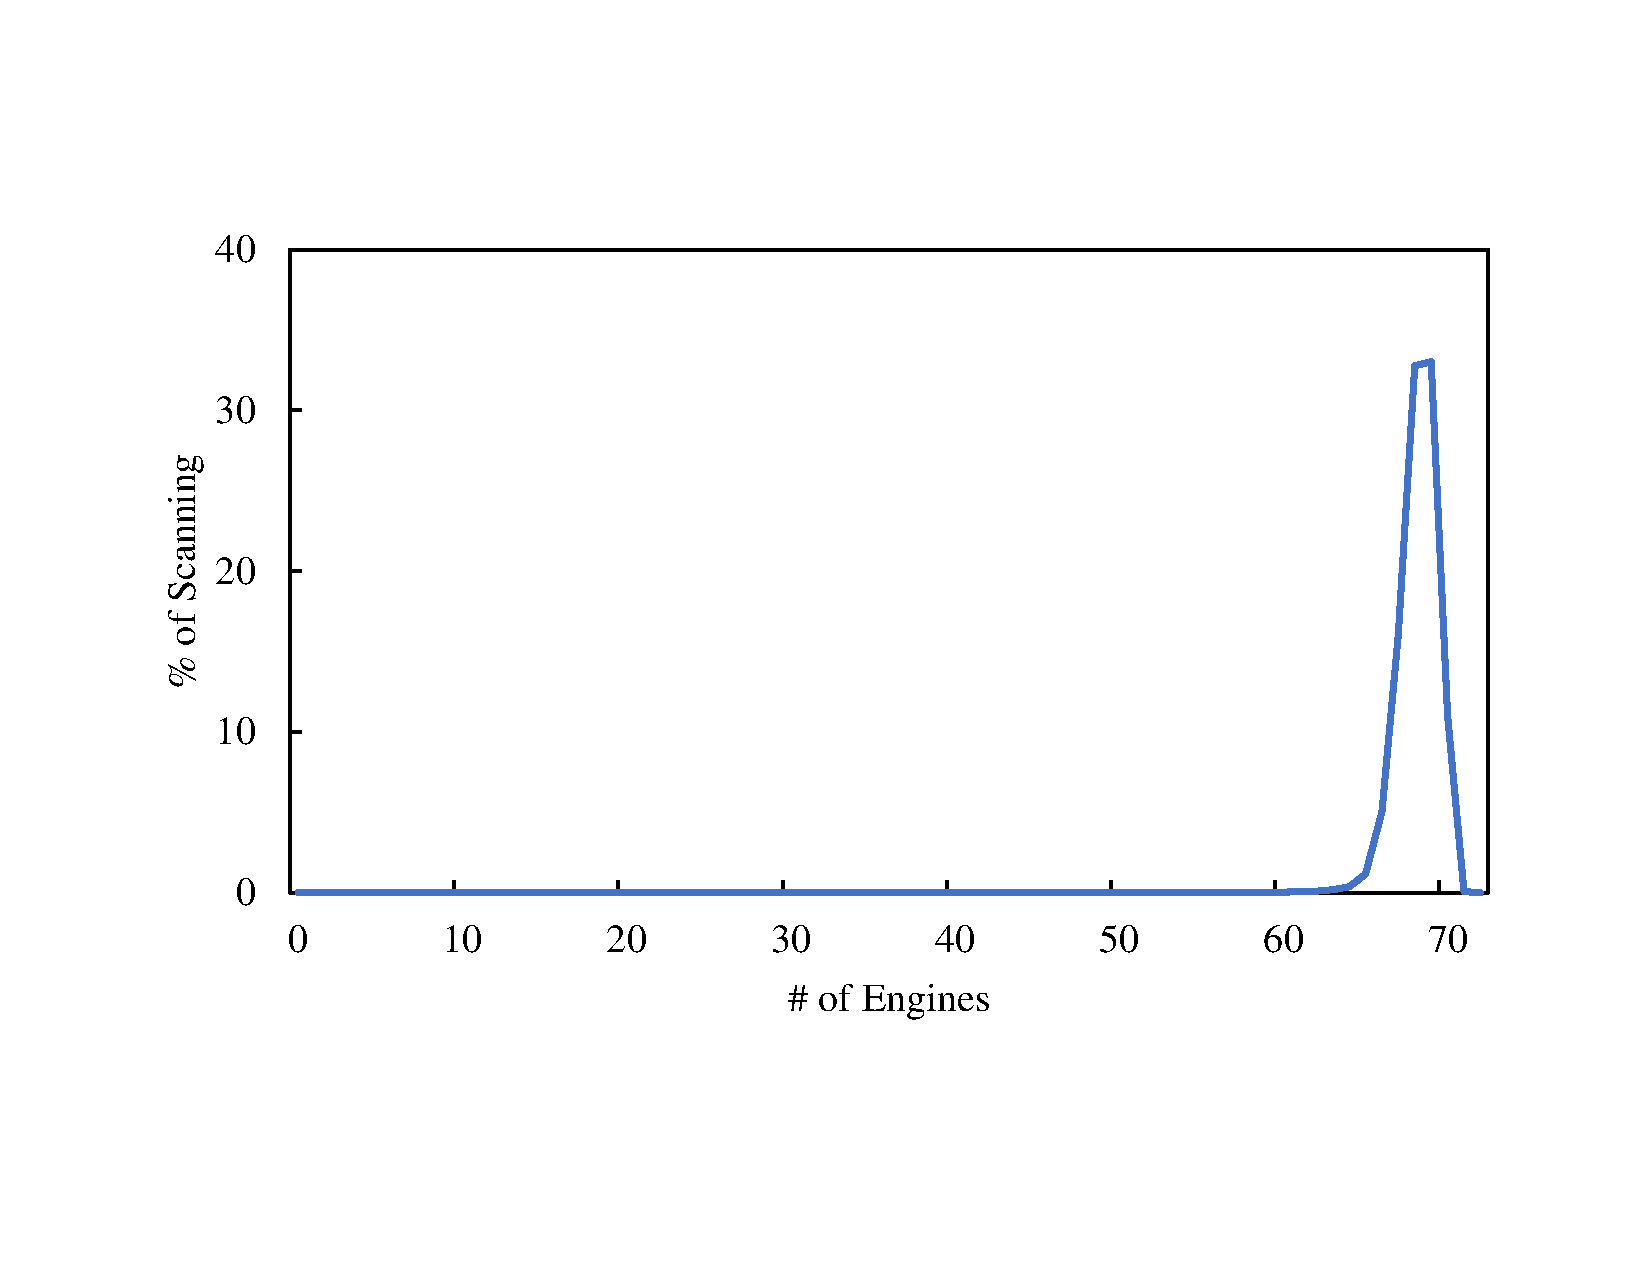
\includegraphics[width=0.7\linewidth]{figure/vendor_submission_distribution}
\caption{Distribution of detection results vs. vendors}
\label{fig:dataset_submission_vendor_distri}
\end{figure}

\begin{figure}
\centering
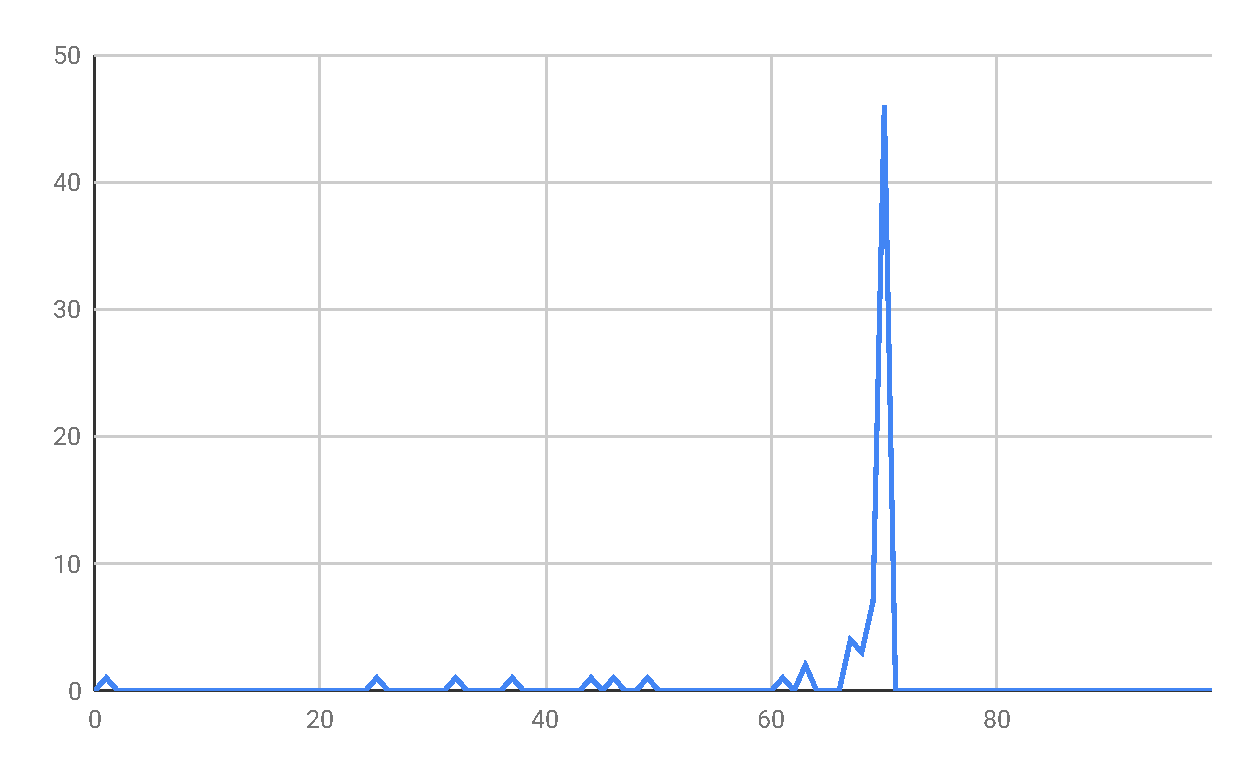
\includegraphics[width=0.7\linewidth]{figure/dataset_no_vendors_scanned_moste_files_in_x_days}
\caption{the number of vendors that scanned more than 12980 (>90\%) files in $x$ days}
\label{fig:dataset_no_vendors_scanned_moste_files_in_x_days}
\end{figure}


\subsection{How VirusTotal update engines?}
As we mentioned above, we use \texttt{rescan} and \texttt{report} to get the latest detection results from VirusTotal for each day. Actually, how VirtusTotal update the antivirus engines? With our data set for 75 days, we first check whether antivirus bases and versions update over time. We find that more than 78\% of the detection results updates consistently with time went on. So we can get new detection results from VirusTotal when we \texttt{rescan} samples and \texttt{report} detction results 2 hours later.


\begin{figure}
\centering
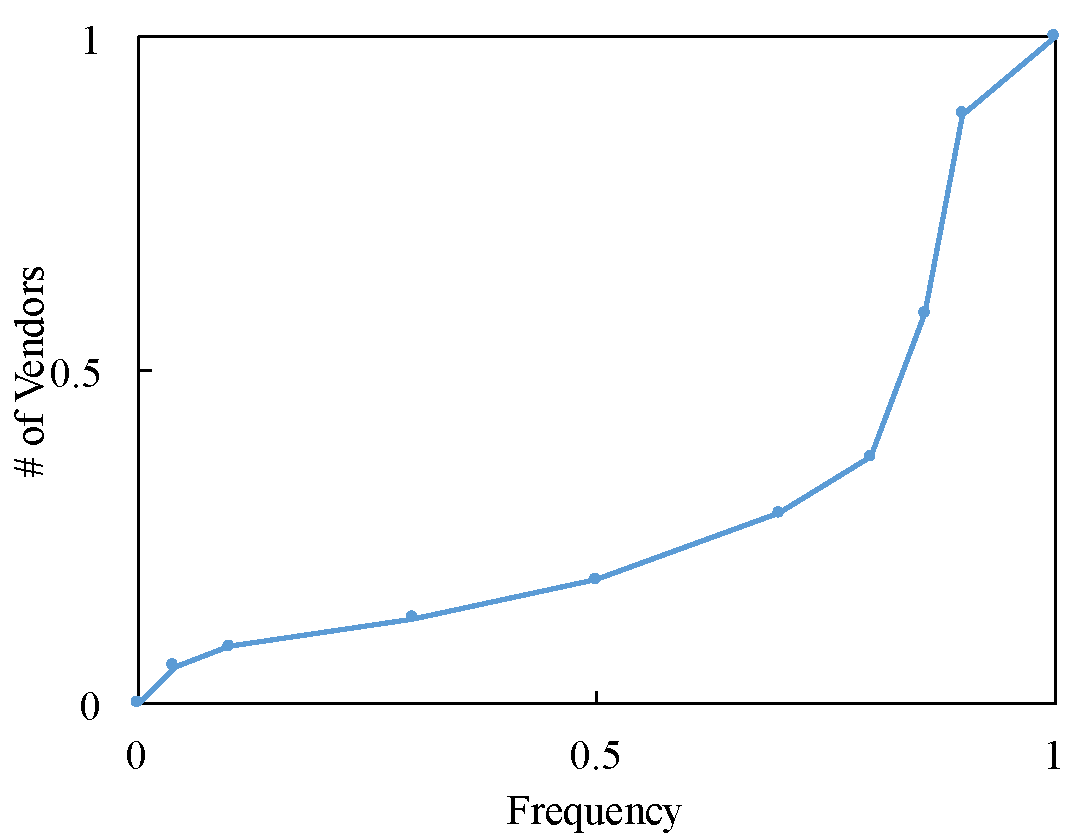
\includegraphics[width=0.7\linewidth]{figure/frequency}
\caption{Distribution of update frequency over vendors.}
\label{fig:frequency}
\end{figure}

Figure \ref{fig:requency} presents the distribution of updating frequency for vendors. Overall, more than 44 vendors(total 70) update their detction results with at least 1 day. Only 6 vendors' updating frequency are less than 0.05, and 4 of them seems not change their antivirus engines during these 75 days. Averagely, about 56 vendors will be updated with at least 2 days. 

%c. How VirusTotal update engines? Scanning time vs. update vs. version 
%TODO: need more data
\subsection{Caveats}

Discuss errors during our data collection. 

\section{Flipping and stable study}

In this section, we present how we analyze our collected data during these 75 days, and try to find some patterns on the detection results of 14423 samples from 70 vendors. 

Based on our obversation, we first give some definitions of different patterns: (1) Stable pattern: This pattern means that the detection results of a file from an vendor or all vendors would never change. (2)Flip pattern: Some vendors will change the detection result of a file from malicious to benign or from benign to malicious one time in the sequence. (3)Hazard pattern: The results would be updated from benign to malicious at one day, and then back to benign again. The same situation would also happen on malicious files. 


\subsection{Hazard discussion}

\begin{figure*}[!htb]
\minipage{0.31\textwidth}
  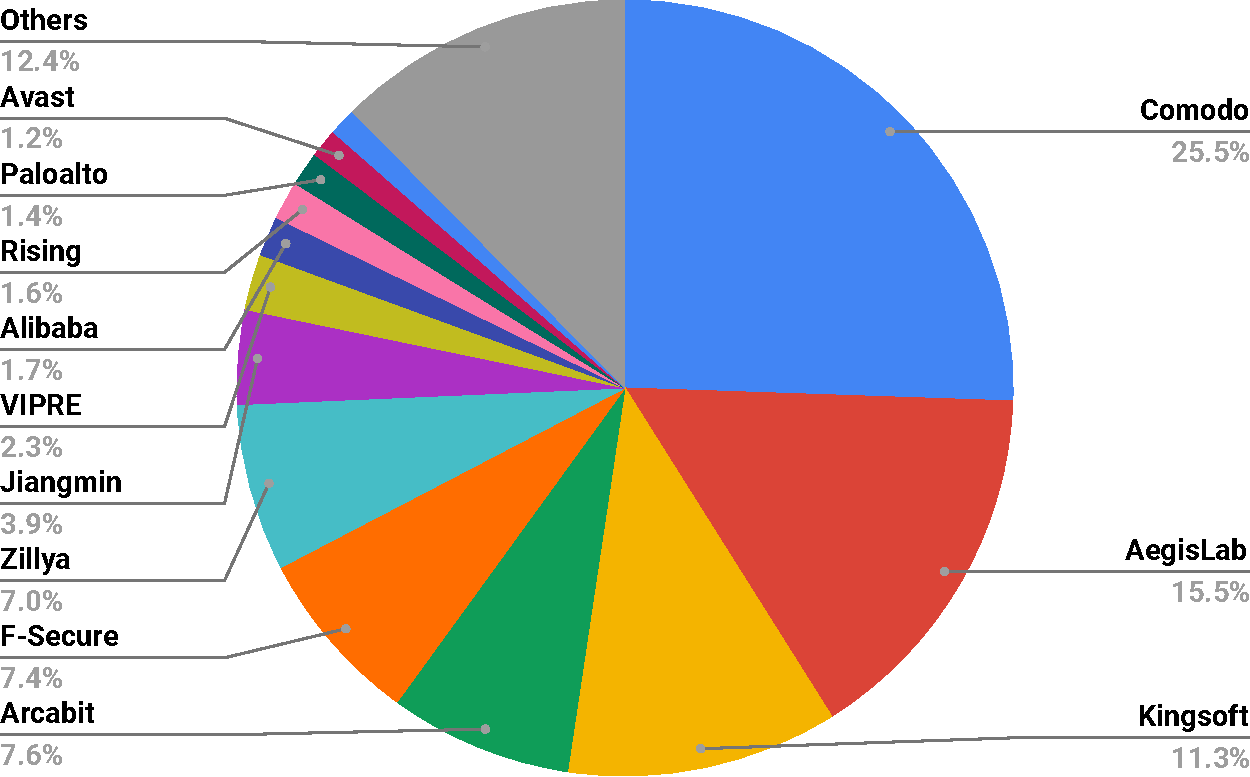
\includegraphics[width=\linewidth]{figure/hazard_vendorAll}
  \caption{Hazard distributions for vendors.
%(File types and their distributions for all VirusTotal submissions from 05/07/2016 to 09/06/2016.)
}
\label{fig:hazard_vendorAll}
  %\label{fig:overlap}
\endminipage\hfill
\minipage{0.31\textwidth}
  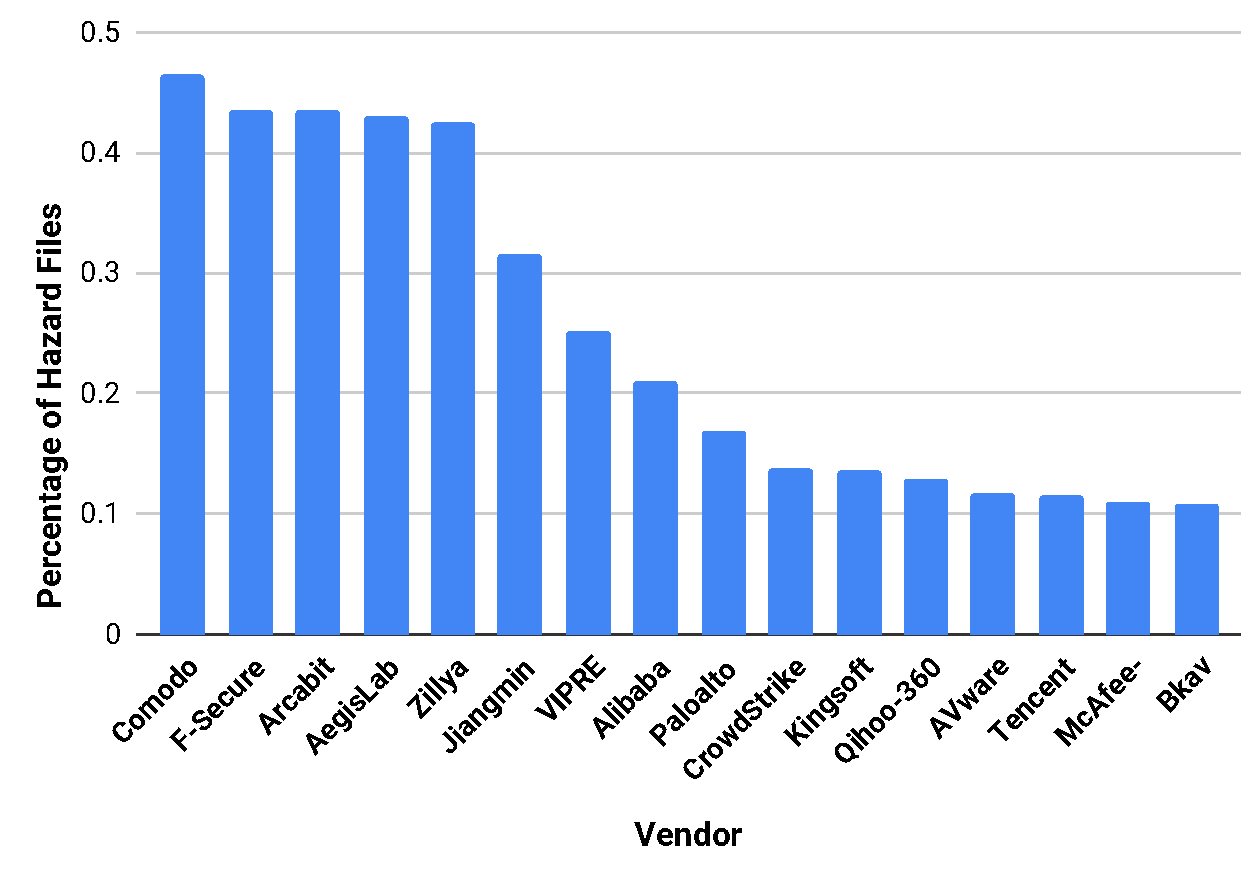
\includegraphics[width=\linewidth]{figure/hazard_vendorFile}
 \caption{Hazard file distributions for per vendor.
%{\footnotesize{
%(The number of suspicious files and the number of PE files submitted to VirusTotal from 05/07/2016 to 09/06/2016.)
%}
}
\label{fig:hazard_vendorFile}
  %\label{fig:maxUncover}
\endminipage\hfill
\minipage{0.31\textwidth}%
  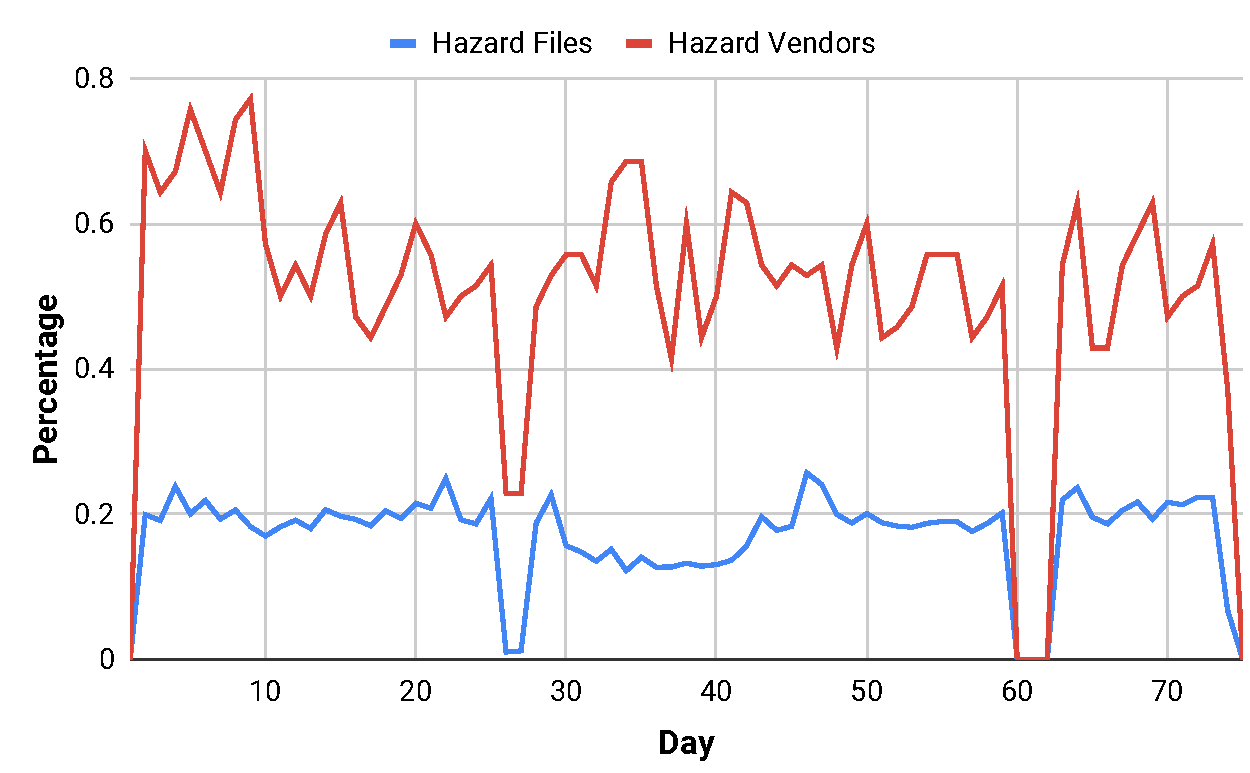
\includegraphics[width=\linewidth]{figure/hazard_day}
\caption{Hazard file and vendor distributions for per day.
%\footnotesize{
%(Only countries with more than 1\% PE submissions are shown.)
%}
}
\label{fig:hazard_day}
\endminipage\hfill

%\vspace{-0.2in}
\end{figure*}

Hazard pattern is an abnormal situation in the dection result sequences. It could affect the study of the other two patterns. So we first caculated the distribution of hazards over vendors, sampling files and days in our original data set.

In our statistics, only 3 vendors have no hazard patterns and other 67 vendors have hazards with different percentage. Hazards from the top 3 vendors accounts half of hazards and 13 vendors can cover more than 87\% hazards. Other 54 vendors have less than 1\% hazards, as shown in Figure \ref{fig:hazard_vendorAll}. Hazard pattern is quite frequently among vendors and sampling files.

Figure \ref{fig:hazard_vendorFile} shows the percentage of hazard files from top 16 vendors. Other vendors contains less than 10\% hazard files. "Comodo" contains the most hazards but has less than half of hazard files. We can make a conclusion from these results that hazard pattern is not caused by the engine misfunction. 

Figure \ref{fig:hazard_day} plots hazards distribution of files and vendors over every day. Overall, we find that hazard files randomly appear almost every day during these 75 days. The same conclusion can be made to hazard vendors. 

Figure \ref{fig:hazard_fileVendor} presents hazard file distribution over vendors. Only 4 hazard files involves more than 30 vendors and we did not find a file that its detection results from 70 vendors have hazard patterns. Thus, hazard pattern may not caused by the VirusTotal API.



%Todo: add hazard discussion in this part before discussing flipping. 

%Hazard caused by VT API? NO

%Hazard caused by vendor misfunction? NO

%conclusion: randomly appear, but quite frequently, affect lots of files

%Conclusion: remove hazard before studying flipping?

%Run experiments both with and without hazard
\textbf{Summary:} Hazard pattern is obviously common in our results and it affects lots of files and vendors. An immediate question that follows is what the results would be if we remove hazards before studying flipping and stable patterns? We will give more explanations of our experiments in the following sections.  

\subsection{Flipping Study}
%a. For each file, we count  of flipping vendors and  of flipping times

\begin{figure*}[!htb]
\minipage{0.31\textwidth}
  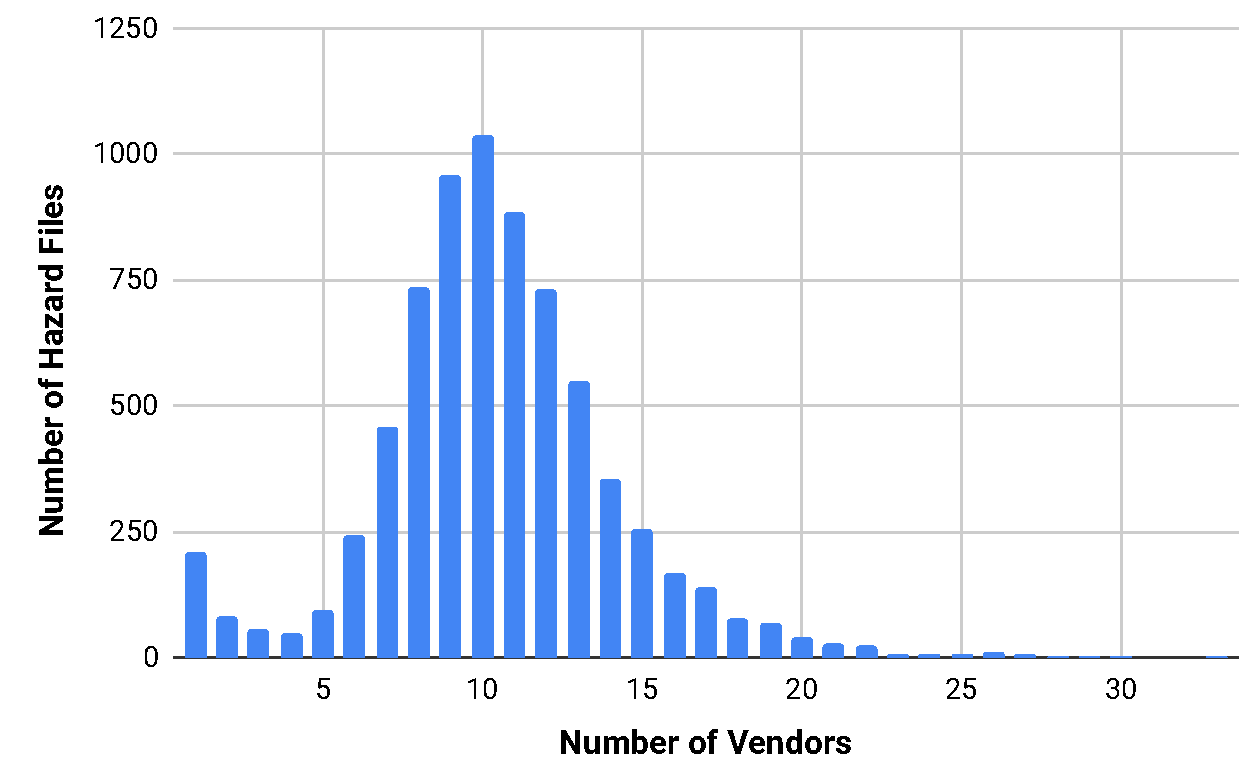
\includegraphics[width=\linewidth]{figure/hazard_fileVendor}
  \caption{Hazard file distributions over vendors.
%(File types and their distributions for all VirusTotal submissions from 05/07/2016 to 09/06/2016.)
}
\label{fig:hazard_fileVendor}
  %\label{fig:overlap}
\endminipage\hfill
\minipage{0.31\textwidth}
  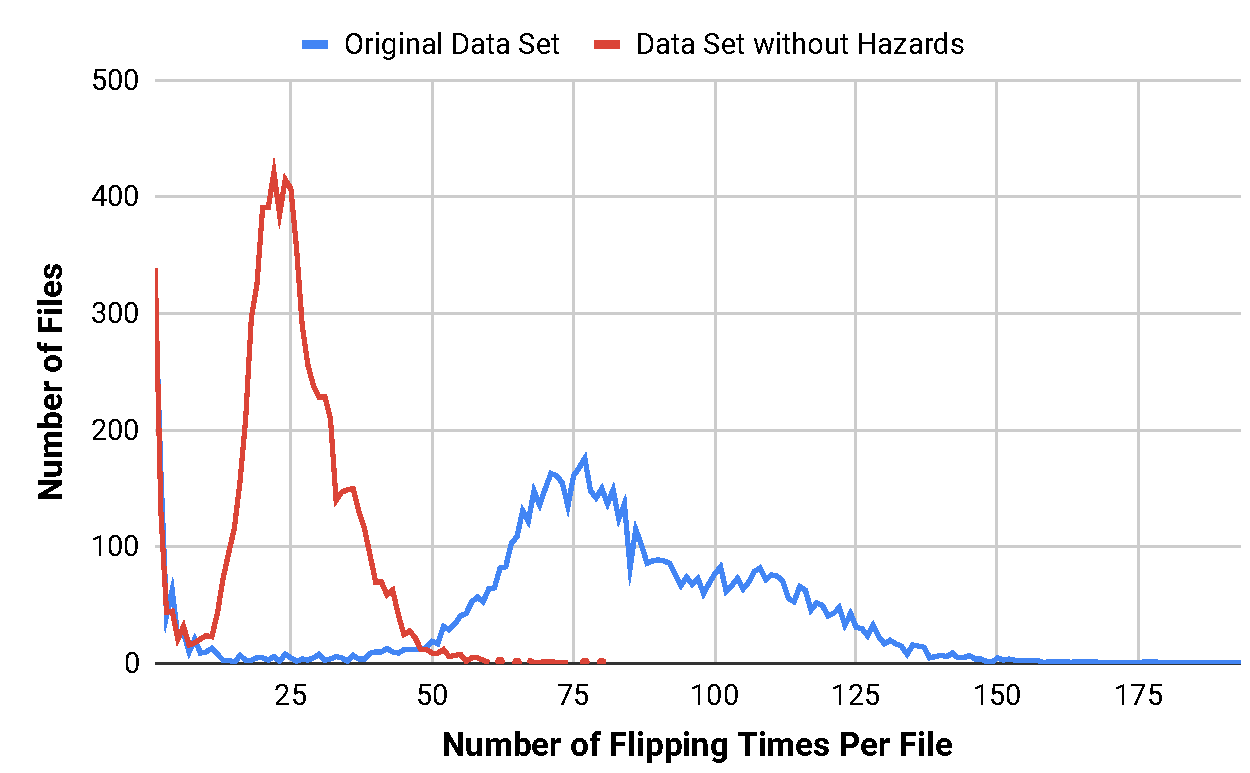
\includegraphics[width=\linewidth]{figure/flip_all}
 \caption{Flipping distributions for per file.
%{\footnotesize{
(The number of flipping times comparisons on data set both with and without hazards.)
%}
}
\label{fig:flip_all}
  %\label{fig:maxUncover}
\endminipage\hfill
\minipage{0.31\textwidth}%
  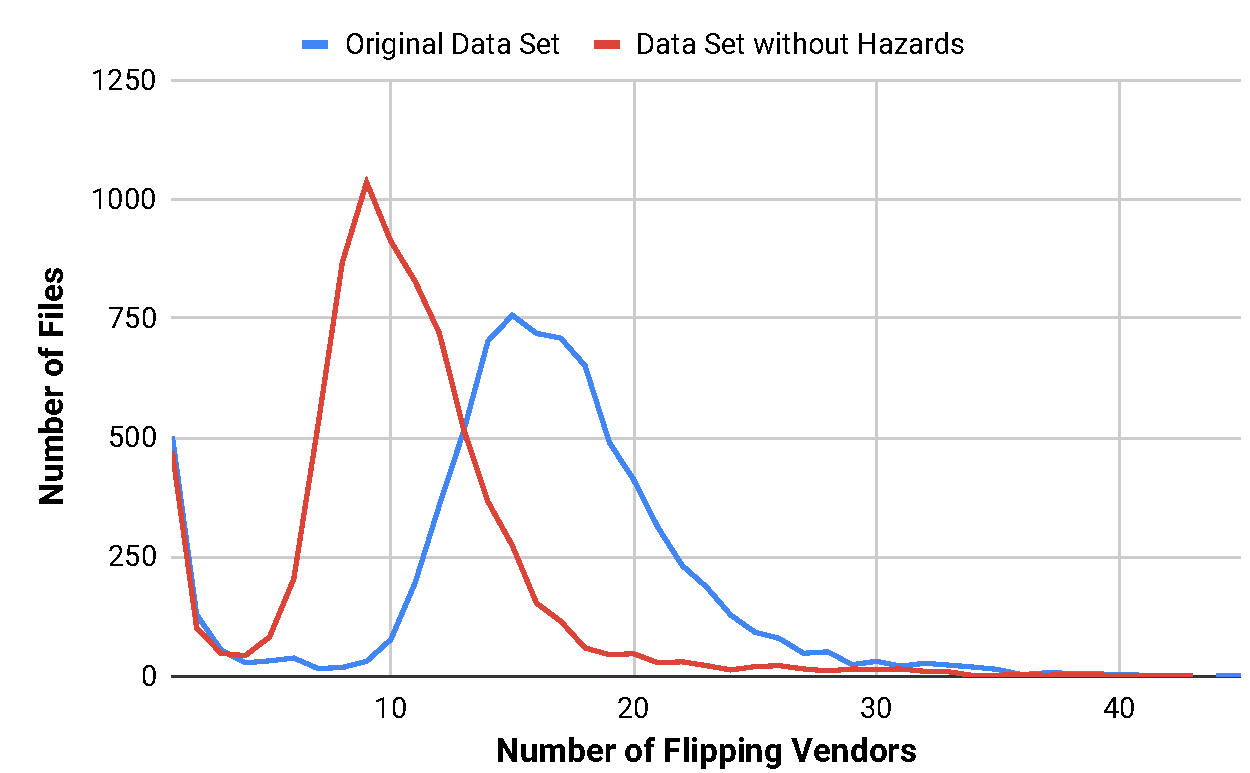
\includegraphics[width=\linewidth]{figure/flip_file}
\caption{Flipping vendor distributions for per file.
%\footnotesize{
(The number of flipping vendors comparisons on data set both with and without hazards.)
%}
}
\label{fig:flip_file}
\endminipage\hfill

%\vspace{-0.2in}
\end{figure*}

This section presents our results of flipping pattern study. As we discussed above, flipping pattern is an important pattern that affects a file to be stable. To study the flipping pattern, we calculate fippling distribution over files and vendors respectively in our original data set. Then, we remove hazards from our data set and recaulate the distributions for further comparison. 

Figure \ref{fig:flip_all} shows the distribution of flipping times for each file. Totally, we find that 7754 files have flipping patterns(total 14423), and the number drops to 7657 after smoothing hazards. Only 1 file have the largest flipping times of 193, and most files have only one flip. Without hazards, the largest flipping times is 80 and most files contian less flippings. For example, more than 421 files contain 22 flipping patterns. We can make the similar conclusion from the distribution of flipping vendors for each file, as shown in Figure \ref{fig:flip_file}. 

%b. For each vendor, we count  of flipping,  of flipping files, average flipping per file

To figure out the distribution of flipping pattern for each vendor, we calculate the flipping times, the number of flipping files from each vendor and the average flipping times per file. We run the same experiments both on our original data set and data set without hazards.

Overall, 68 vendors have flipping patterns(total 70), and "Comodo" contains more flipping patterns than other vendors. Some vendors, such as "Avast-Mobile" and "eGambit", have no flippings during the detction period. We present top 16 vendors ranking in the flipping list in Figure \ref{fig:flip_vendorAll}. Compared with results from the original data set, removing hazards has greatly reduced the flipping times for each vendor. 

Figure \ref{fig:flip_vendorFile} shows the distribution of flipping files for each vendor. 7 vendors have more than 40 percentage fippling files(total 14423). Removing hazards almostly does not affect the number of flipping files of some vendors. For some vendors, such as "Acrabit", "Zillya", "F-Secure", "CrowdStrike", we find the number of flipping files dramatically drops when we remove hazards from the original data set.

Figure \ref{fig:flip_vedorAvg} plots the average flipping times of a file from each vendor. We present 28 vendors that have more than 2 flipping times per file averagely, while other 42 vendors hold less than 2 flippings for each file. The most frequent flipping happens on "Comodo". On average, it contains more than 30 flipping times per file. Without hazards, the average flipping times significantly fall into almost half of original results. 

\begin{figure*}[!htb]
\minipage{0.31\textwidth}
  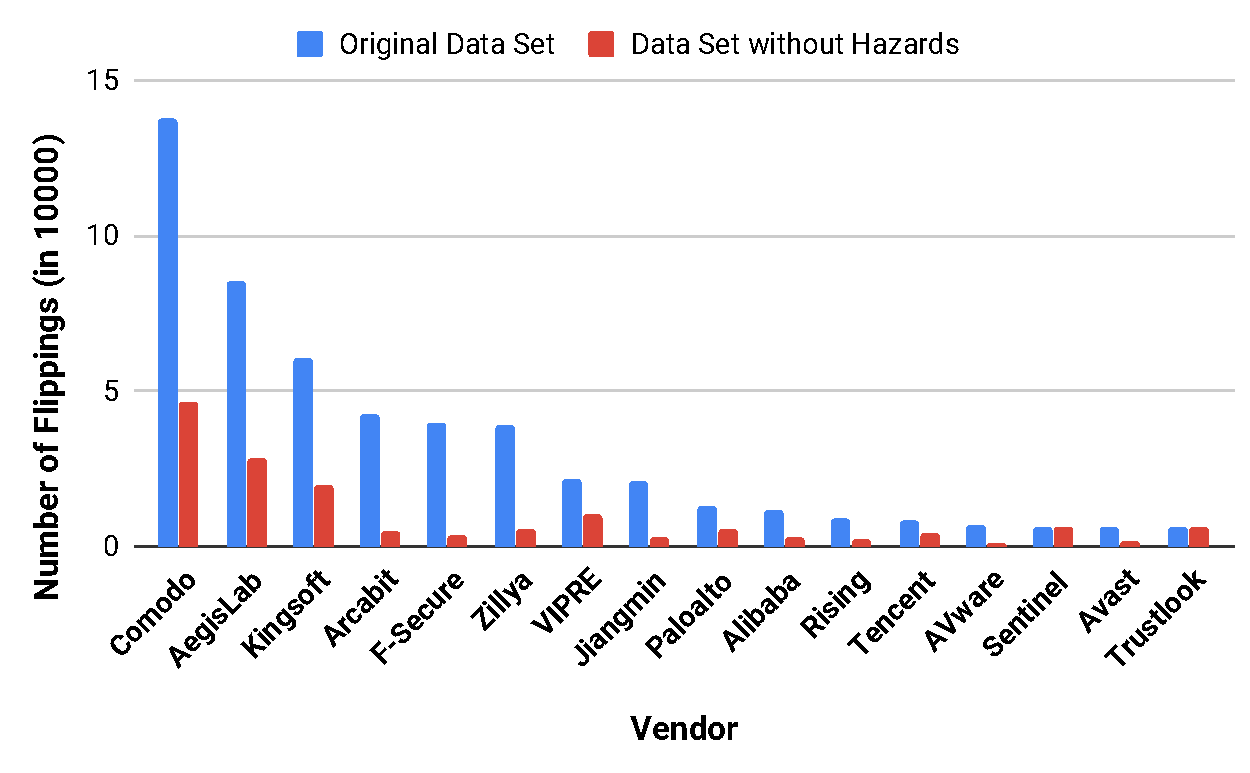
\includegraphics[width=\linewidth]{figure/flip_vendorAll}
  \caption{Flipping distributions for vendors.
(The number of flipping times for per vendor comparisons with and without hazards.)
}
\label{fig:flip_vendorAll}
  %\label{fig:overlap}
\endminipage\hfill
\minipage{0.31\textwidth}
  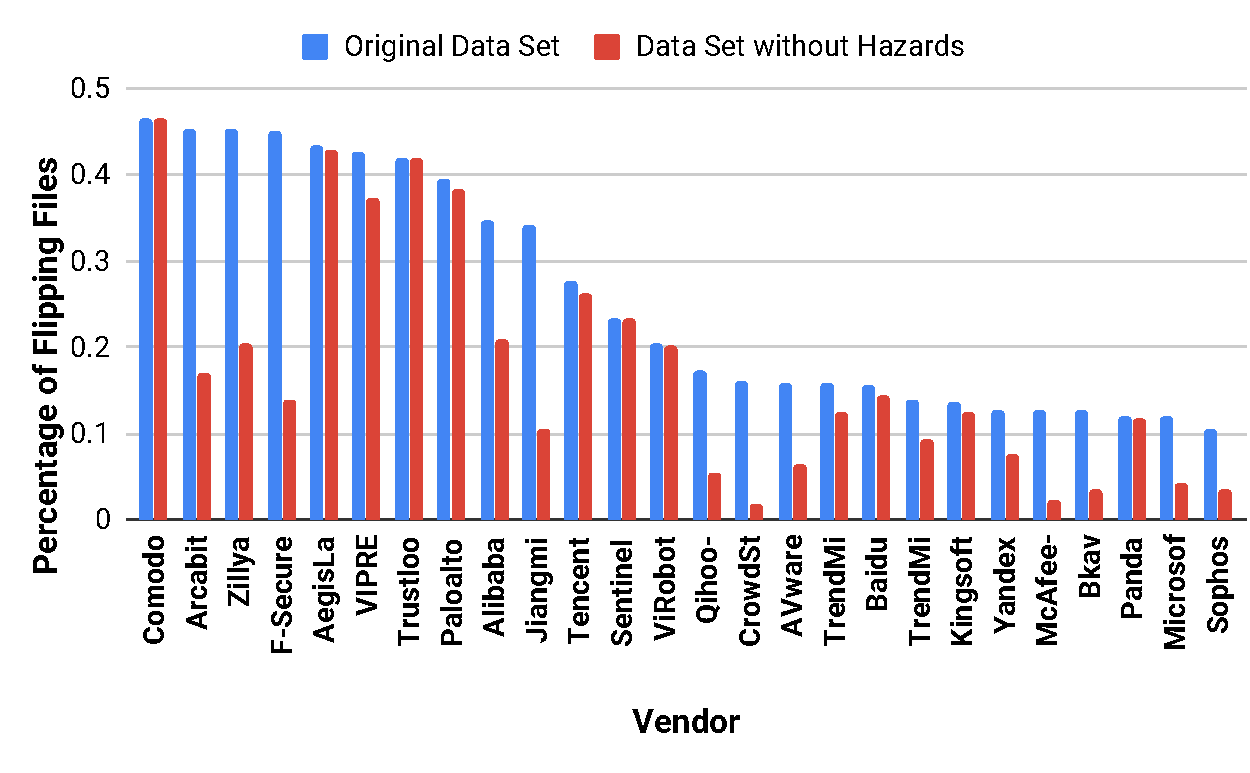
\includegraphics[width=\linewidth]{figure/flip_vendorFile}
 \caption{Flipping file distributions for per vendor.
%{\footnotesize{
(The number of flippings files for per vendor comparisons with and without hazards.)
%}
}
\label{fig:flip_vendorFile}
  %\label{fig:maxUncover}
\endminipage\hfill
\minipage{0.31\textwidth}%
  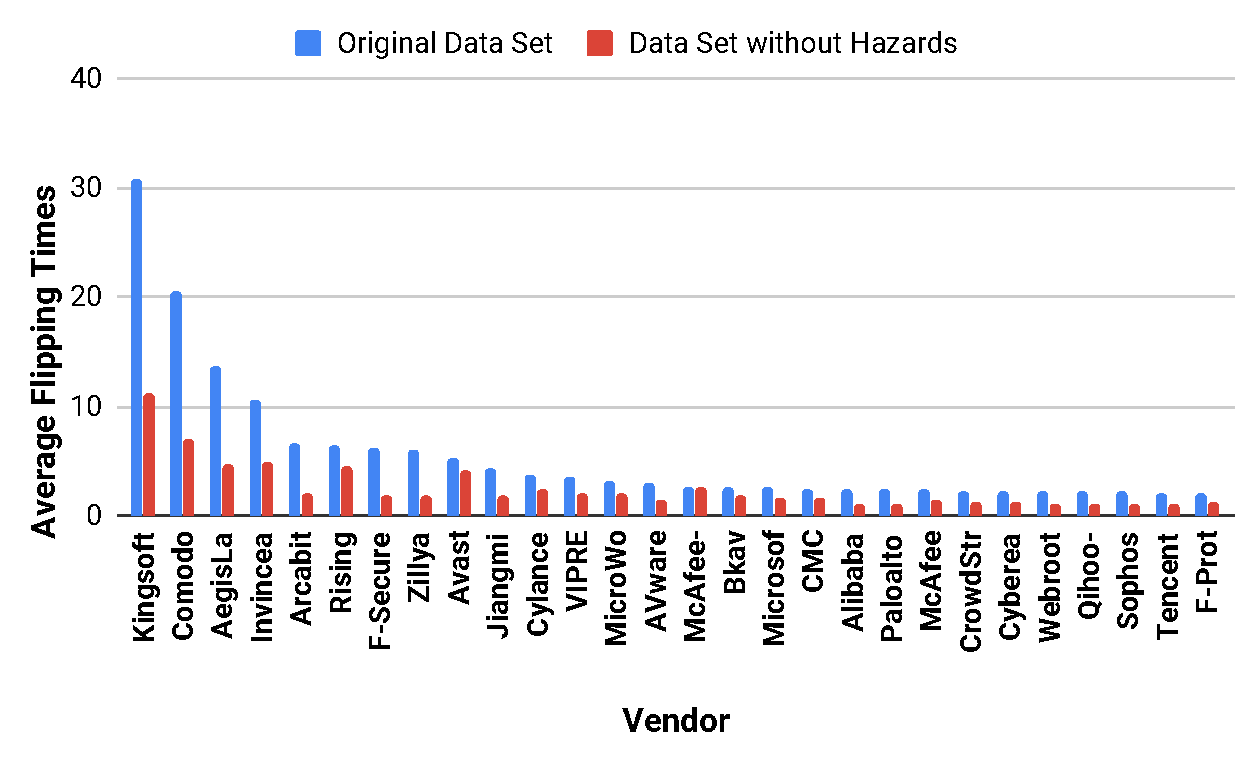
\includegraphics[width=\linewidth]{figure/flip_vendorAvg}
\caption{Average flipping times of a file for per vendor.
%\footnotesize{
(The average flipping times of a file for per vendor comparisons with and without hazards.)
%}
}
\label{fig:flip_vedorAvg}
\endminipage\hfill

%\vspace{-0.2in}
\end{figure*}

\textbf{Summary:} Flipping pattern widely exists in our experiments. Statistically, more than 50\% files and 97\% vendors have flipping patterns. Removing hazards is an effective approach to reduce flipping patterns for some vendors, but only 97 files have no flipping pattern after smoothing hazards. A large numbers of files and vendors still have flipping patterns. Flipping pattern is the most important reason that results in many files and vendors to be unstable.


\subsection{Stable Study}
a. We need some metrics to support our definition of ?stable? is reasonable.

b. Some metrics to show how long we need to wait until results become stable

\subsection{Conclusions}

\section{Influence model}

%\subsection{Influence graph}

\textcolor{gray}{How we model vendors? influence}

As we have mentioned in Section (blah), vendors could rely on each other to decide their own detection results. 
To measure such influence among vendors, we adapt the static influence model on social networks by Goyal et al. \cite{goyal2010learning}. 
Their model calculates influences among nodes in a social network based on chronological relationships of the actions they have taken.
The influences are probabilities of how one node could affect another.

In this paper, there 3 main differences from the original model. 
\begin{itemize}
	\item First, we do not have a graph that explicitly shows how vendors connects with each other. 
	We assume that each vendor could influence any other vendors, and calculate the influence on a complete graph. 
	\item Second, we do not know the exact time point that a vendor executes an action: we only have many time series of detection results. 
	We assume that when detection results of a sample change, the vendor executes an action.
	\item Third, an action could be executed by a vendor more than once in our scenario, while the original model only allows an action to be executed by a node only once. 
	This makes it hard to decide which and how many execution(s) of an action influences another, which is important to decide how to calculate the probabilities.
	In this paper, we assume that an execution is only affected by only one another execution per vendor.
	We also adjusted the method of calculating the probabilities. We enlarge the event space so that when actions are executed multiple times, the probabilities could be calculated reasonably. 
	
\end{itemize}

%One important problem in this scenario is that we should decide when there are multiple executions of an action, 
%In the original model, this would cause the probabilities larger than 1.

Now we introduce our model. First, we sample almost everyday for each sample, and get more than 70 vendors' detection results. 
For a vendor $v$, it could mark a file $f$ as malicious or benign at some day $d$. 
We denote the sampling result `marking as malicious' as $(v, f_1, d) \in S$ and `marking as benign' as $(v, f_0, d) \in S$. 
As we have mentioned, when the detection result of $v$ flips from benign to malicious, we consider it as an action is performed. We write 
\[flip(v, f, d) = \exists d' d=prev(v, f, d) \land (v, f_0, d') \land (v, f_1, d) \] 
to indicate that vendor $v$ flips its detection result on sample file $f$ at day $d$, where $prev(d)$ represents the previous day that we sampled: 
\[prev(v, f, d) = \max \{d| (v, f_0, d)\in S \lor (v, f_1, d)\in S\}\]

When a flip happens, we consider how the vendor learns from other vendors. The vendor $v$ could learn from another vendor $u$, where there are a sampling $(u, f_1, d_u)$ that $d_u < d$. In this case, we consider vendor $u$ affects vendor $v$. 
We define the set of actions propagated from $u$ to $v$ as follows:
\begin{equation}
A_{u2v} = \{(v, f_1, d)| \exists (u, f_1, d_u)\in S. flip(v, f, d) \land d_u<d \}
\end{equation}

When calculating the probabilities of the influence model, $|A_{u2v}|$ is used as the nominator. 
We adjusted the denominator to ensure that the probability is no more than 1.
Different from the original model where they use all the actions of $u$ as the event space, here we use the samplings as the event space and take it as the denominator, since the number of flips must less than the number of samplings.
First we define the event space of vendor $u$ as:
\[
S_u = \{(u, f_*, d)|(u, f_*, d) \in S\}
\]
Then we also consider the number of samplings of $u$ and $v$ in common:$S_{u|v}$. For convenience, we calculate as follows: \[|S_{u|v}|=|S_u|+|S_v|-|S_{u\&v}|\] For $S_{u\&v}$, we have:
\[
S_{u\&v} = \{(u, f_*, d)| (u, f_*, d)\in S_u \land \exists (v, f_*, d)\in S_v \}
\]

%\subsection{Basic Definitions}
%First, we introduce some basic definitions of actions. 
%, and how to generate an action $(v, a , t)$ or actions in action list $Actions$ from a time sequence $s$. 
%\textcolor{red}{Currently, we consider all the detection results in each day as an action. Should we eliminate some of the actions?}

%Then we define action propagation among vendors. 
%We denote $prop(a, v_i, v_j, \Delta d)$ as ``an action $a$ propagates from $v_i$ to $v_j$ in $\Delta d$ days'', where $\Delta d = d_j-d_i$. 
%This happens iff. $\exists (v_i, a, d_i), (v_j, a, d_j) \in Actions$ with $d_j-d_i>d_w$, where $d_w$ is the time window of vendors reference other vendors. \textcolor{red}{We would like to know the results under different time windows.} 

%Now we define how to calculate the influence among vendors. 
%We write $A_v$ as the number of actions performed by vendor $v$. 
%Formally, we have 
%\begin{equation}
%A_v = |\{(u, a, d) | (u, a, d) \in Actions \land u=v\}| 
%\end{equation}

%Then, we consider the actions that two vendors $u$ and $v$ performed together: 
%\begin{multline}
%A_{u\&v} = |\{(u, a, d) | (u, a_u, d_u) \in Actions \\ \land (v, a_v, d_v) \in Actions \land a_u=a_v \}|
%\end{multline}

%The number of actions that performed by either vendors could be calculated as: 
%\begin{equation}
%A_{u|v} = A_u+A_v-A_{a\&v}
%\end{equation}

%We also have 
%\begin{multline}
%A_{u2v} = |\{(u, a_u, d_u) | (u, a_u, d_u) \in Actions \\ \land (v, a_v, d_v) \in Actions \land a_u=a_v \land d_u<d_v \}|
%\end{multline}
% as the number of actions propagated from $u$ to $v$. 

%With the values, we could calculate the influences, which is defined on a complete graph $G= (V,E)$. $V$ is the set of vendors, and $\forall u,v \in V, \exists (u,v,p_{u,v}) \in E$, where 
%$p_{u,v}$ is the influence probability of $v$ influenced by $u$. 

\subsection{Influence measurement}
We have 4 metrics of calculating probability $p_{u,v}$ as follows:

\textbf{Bernoulli Distribution:} This model estimates $p_{u,v}$ as the ratio of the number of actions propagated from $u$ to $v$ over the total number of actions taken by $u$.

\begin{equation}
p_{u,v} = \frac{|A_{u2v}|}{|S_u|}
\end{equation}

\textbf{Jaccard Index:} This model estimates $p_{u,v}$ as the ratio of the number of actions propagated from $u$ to $v$ over the total number of actions taken by either $u$ or $v$.

\begin{equation}
p_{u,v} = \frac{|A_{u2v}|}{|S_{u|v}|}
\end{equation}

We also consider partial credit to improve the two metrics above.
The partial credit is explained as follows. When $v$ takes an action $a$, it may be influenced by the combination of all its neighbors taking the action $a$ before $v$. To account for this effect, we use partial credit and calculate the partial credit for $u$ who takes an action $a$ before $v$ as

\begin{equation}
%A_{u2v} = \{(v, f_1, d)| \exists (u, f_1, d_u)\in S. flip(v, f, d) \land d_u<d \}
credit(f_1, d) = \frac{1}{\sum_{w \in V}I(\exists (w, f_1, d_w) \in S \land d_w<d}
\end{equation}

where $V$ is the set of vendors and $I$ is the indicator: $I(P)$ equals to 1 when $P$ is true, otherwise it is 0. Then we have another two metrics:

\textbf{Bernoulli Distribution with Partial Credit:} This model estimates $p_{u,v}$ as the sum of all partial credits taking by u for actions propagated from $u$ to $v$, dividing by the number of actions taken by $u$.

\begin{equation}
p_{u,v} = \frac{\sum_{(v,f_1,d)\in A_{u2v}}credit(f_1, d)}{|S_{u}|}
\end{equation}

\textbf{Jaccard Index with Partial Credit:} This model estimates $p_{u,v}$ as the sum of all partial credits taking by u for actions propagated from $u$ to $v$, dividing by the number of actions taken by $u$.

\begin{equation}
p_{u,v} = \frac{\sum_{(v,f_1,d)\in A_{u2v}}credit(f_1, d)}{|S_{u|v}|}
\end{equation}

%How we generate the dataset is illustrated as in Figure \ref{fig:action}. In this figure, there are three vendors, $u$, $v$, and $w$. $v$ flips at time 4 and 9, from benign to malicious. $w$ flips from benign and malicious at time 5. For $v$, it could be influenced by $u$ at time 3 and time 8, and $w$ at time 8. For $w$, it could be influenced by both $u$ and $v$ at time 8. Therefore, for this small case, we have the following action propagations: $(u, f_1, 3) \to (v, f_1, 4)$, $(u, f_1, 8) \to (v, f_1, 9)$, and $(w, f_1, 8) \to (v, f_1, 9)$.
\textcolor{red}{malicious to benign is easy to calculate. We can calculate all the probabilities among vendors and have a complete graph. We illustrate the sum of edges and heatmap. Also some vendor pairs with high impact.}
\subsection{Results}

A heatmap illustrated in one figure

a. On the small data set

b. On the large data set**

Justify file category

Justify length of the data

\subsection{Discussion}

\section{Prediction Model}

\subsection{Overview}

What do we want to predict?

a. Whether a file is stable now

b. decision tree

\subsection{Experiments and implications}


\section{Related works}

The AISec Paper

\section{Conclusions}


%%\balance
%\begin{spacing}{0.65}

\balance
{
\bibliographystyle{ACM-Reference-Format}
\bibliography{security}

}
%\end{spacing}
\end{document}
